\subsection{The target class cannot be duplicate with any existing class within same package after rename.}

When we try to rename a class with an existing class name, the Eclipse produces syntax error:
``Please choose another name".~\cite{EclipseWebPage} The classes will be conflicted if we rename the target class using the name of an existing class in the same package. So we can not have duplicate class names in the same package. 

For example, a package \textsl{p} contains class: \textsl{A}, \textsl{B} and \textsl{C}, now we want to refactor the class name \textsl{A} to \textsl{B}:

\begin{figure}[th]
\centering
\begin{minipage}[t]{0.35\linewidth}
\begin{lstlisting}[language=java, basicstyle=\scriptsize\ttfamily,frame=single]
package p;

class A{}	
class B{}
class C{}
\end{lstlisting}
\tiny{(a) Before Rename Refactoring Class A}
\end{minipage}
\hfill
\begin{minipage}[t]{0.35\linewidth}
\begin{lstlisting}[language=java, basicstyle=\scriptsize\ttfamily,frame=single]
package p;

class B{}	
class B{}
class C{}

\end{lstlisting}
\tiny{(b) After Rename Refactoring Class A}
\end{minipage}
\caption{Example of Rename Class Refactoring}
\label{fig:afterrr}
\end{figure}

Then the java compiler shows up the error that B.java already exists as figure \ref{fig:renameclassname}:

\begin{figure}[H]
\centerline{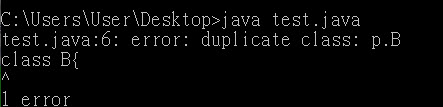
\includegraphics[width=85mm,scale=0.5]{SCN.jpg}}
\caption{The error of using same class name for refactoring}
\label{fig:renameclassname}
\end{figure}

This precondition is applicable even if one or the other file is empty. So checking whether a class with the same name already exists in a package should be the first job we have to do for rename refactoring. 
